%% %% %% %%
%%
%% Parte A de la práctica
%%
%% %% %% %%

\documentclass[../procedimientos.tex]{subfiles}
\graphicspath{{\subfix{../../images/}}}

\begin{document}
\clearpage
\subsection{Parte A}
\subsubsection{Instrucciones}
Diseñe un circuito digital con compuertas que funcione de la siguiente forma:
Cuando $C$ se coloca en bajo se debe detectar y señalizar, con un diodo led de 
color verde, todos los números divisibles entre cuatro; el led rojo no debe 
encender. Si $C$ cambia a un nivel alto, entonces se debe detectar y 
señalizar, con un led de color rojo, todos los números divisibles entre tres 
y, además, con el led verde, los números divisibles por cinco. El conjunto de 
números es de 4 bits.
\begin{figure}[H]
  \centering
  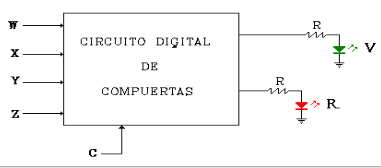
\includegraphics[width=0.5\textwidth]{a_instruction}
  \caption{Ejercicio A}
  \label{fig:a_inst}
\end{figure}

\subsubsection{Análisis}\label{subs:analisis_a}
Antes de comenzar a diseñar la solución para este problema, se requiere 
obtener una función lógica que describa el comportamiento indicado en la 
descripción del problema. Para esto, se asumirá que las funciones buscadas son 
$R(cwxyz)$ para el LED rojo y $V(cwxyz)$ para el LED verde; la cadena $cwxyz$ 
es la representación en bits del número a identificar. El análisis se puede 
comenzar a través de las tablas de verdad de las funciones solicitadas; sin 
embargo, se necesitarían analizar las 32 posibles combinaciones para las 
entradas. Se optó por deducir las formas canónicas \textit{SOP} (Suma de 
Productos, por sus siglas en inglés) de forma inmediata con los casos de 
solicitados.

Primero, para el caso del LED verde, se tienen que marcar todos los 
\textbf{números divisibles entre cuatro} que tienen $C=0$. Los números a 
anlizar son exclusivamente: $0$, $4$, $8$, $12$. De igual forma, se deben 
marcar los \textbf{números divisibles entre cinco} que tienen $C=1$, los 
cuales se listan a continuación: $20$, $25$ y $30$. Con esto, la forma normal 
\textit{SOP} se puede deducir de la siguiente forma:
\begin{equation*}
  V(cwxyz) = \sum_m (0, 4, 8, 12, 20, 25, 30)
\end{equation*}

Desarrollando la suma de productos para simplificar la expresión, se tiene:
\begin{align*}
  V(cwxyz) &= \nt{c}\nt{w}\nt{x}\nt{y}\nt{z} + \nt{c}\nt{w}x\nt{y}\nt{z} + 
  \nt{c}w\nt{x}\nt{y}\nt{z} + \nt{c}wx\nt{y}\nt{z} + c\nt{w}x\nt{y}\nt{z} + 
  cw\nt{x}\nt{y}z + cwxy\nt{z}\\
  &= \nt{c}\nt{y}\nt{z} (\nt{w}\nt{x} + \nt{w}x + w\nt{x} + wx) + 
  c\nt{w}x\nt{y}\nt{z} + cw\nt{x}\nt{y}z + cwxy\nt{z}\\
  &= \nt{c}\nt{y}\nt{z} (1) + c\nt{w}x\nt{y}\nt{z} + cw\nt{x}\nt{y}z + 
  cwxy\nt{z}\\
  &= \nt{c}\nt{y}\nt{z} + c\nt{w}x\nt{y}\nt{z} + cw\nt{x}\nt{y}z + 
  cwxy\nt{z}\\
  &= \nt{c}\nt{y}\nt{z} + c\nt{w}x\nt{y}\nt{z} + cw\nt{x}\nt{y}z + 
  cwxy\nt{z}\\
  &= \nt{c}\nt{y}\nt{z} + cx\nt{z} (\nt{w}\nt{y} + wy) + cw\nt{x}\nt{y}z\\
  &= \nt{c}\nt{y}\nt{z} + cx\nt{z} (w \odot y) + cw\nt{x}\nt{y}z
\end{align*}
\begin{equation*}
  \boxed{
    \therefore V(cwxyz) = \nt{c}\nt{y}\nt{z} + cx\nt{z} (w \odot y) + 
  cw\nt{x}\nt{y}z
  }
\end{equation*}

Por otra parte, para el caso del LED rojo, se tienen que marcar todos los 
\textbf{números divisibles entre tres} que tienen $C=1$, la lista se muestra a 
continuación: $18$, $21$, $24$, $27$ y $30$. Con esto, es posible colocar 
$R(cwxyz)$ en su forma canónica \textit{SOP}, tal como se muestra a 
continuación:
\begin{equation*}
  R(cwxyz) = \sum_m (18, 21, 24, 27, 30)
\end{equation*}

Desarrrollando la suma de productos para simplificar la expresión, se tiene:
\begin{align*}
  R(cwxyz) &= c\nt{w}\nt{x}y\nt{z} + c\nt{w}x\nt{y}z + cw\nt{x}\nt{y}\nt{z} + 
  cw\nt{x}yz + cwxy\nt{z}\\
  &= c(\nt{w}\nt{x}y\nt{z} + \nt{w}x\nt{y}z + w\nt{x}\nt{y}\nt{z} + w\nt{x}yz 
  + wxy\nt{z})\\
  &= c(\nt{x}\nt{z}(\nt{w}y + x\nt{y}) + \nt{w}x\nt{y}z + w\nt{x}yz + 
  wxy\nt{z})\\
  &= c(\nt{x}\nt{z}(\nt{w}y + x\nt{y}) + \nt{w}x\nt{y}z + wy(\nt{x}z + 
  x\nt{z}))\\
  &= c(\nt{x}\nt{z}(w \oplus y) + \nt{w}x\nt{y}z + wy(x \oplus z))
\end{align*}
\begin{equation*}
  \boxed{
    \therefore R(cwxyz) = c(\nt{x}\nt{z}(w \oplus y) + wy(x \oplus z) + 
    \nt{w}x\nt{y}z)
  }
\end{equation*}

\subsubsection{Implementación en Quartus}\label{subs:a_imp}
La implementación en la plataforma \textit{Quartus II} del sistema anterior se 
dividió en símbolos separados. Por un lado

\end{document}

